\begin{fact}
    $\forall (a;b) \in ( \RRsp )^2$,
    $\ln(a b) = \ln a + \ln b$.
\end{fact}


\begin{proof}
    Par définition de $\ln$, nous avons
    $\ln(a b) = \ln a + \integrate*{\frac1t}{t}{a}{ab}$
    (voit le \reffact{int-rdc}).
    %
    Analysons $\setproba{I}_{\,a}^{\,ab} = \integrate*{\frac1t}{t}{a}{ab}$.
    Pour cela, considérons la situation graphique suivante où $1 < a < b$.

    \begin{center}
        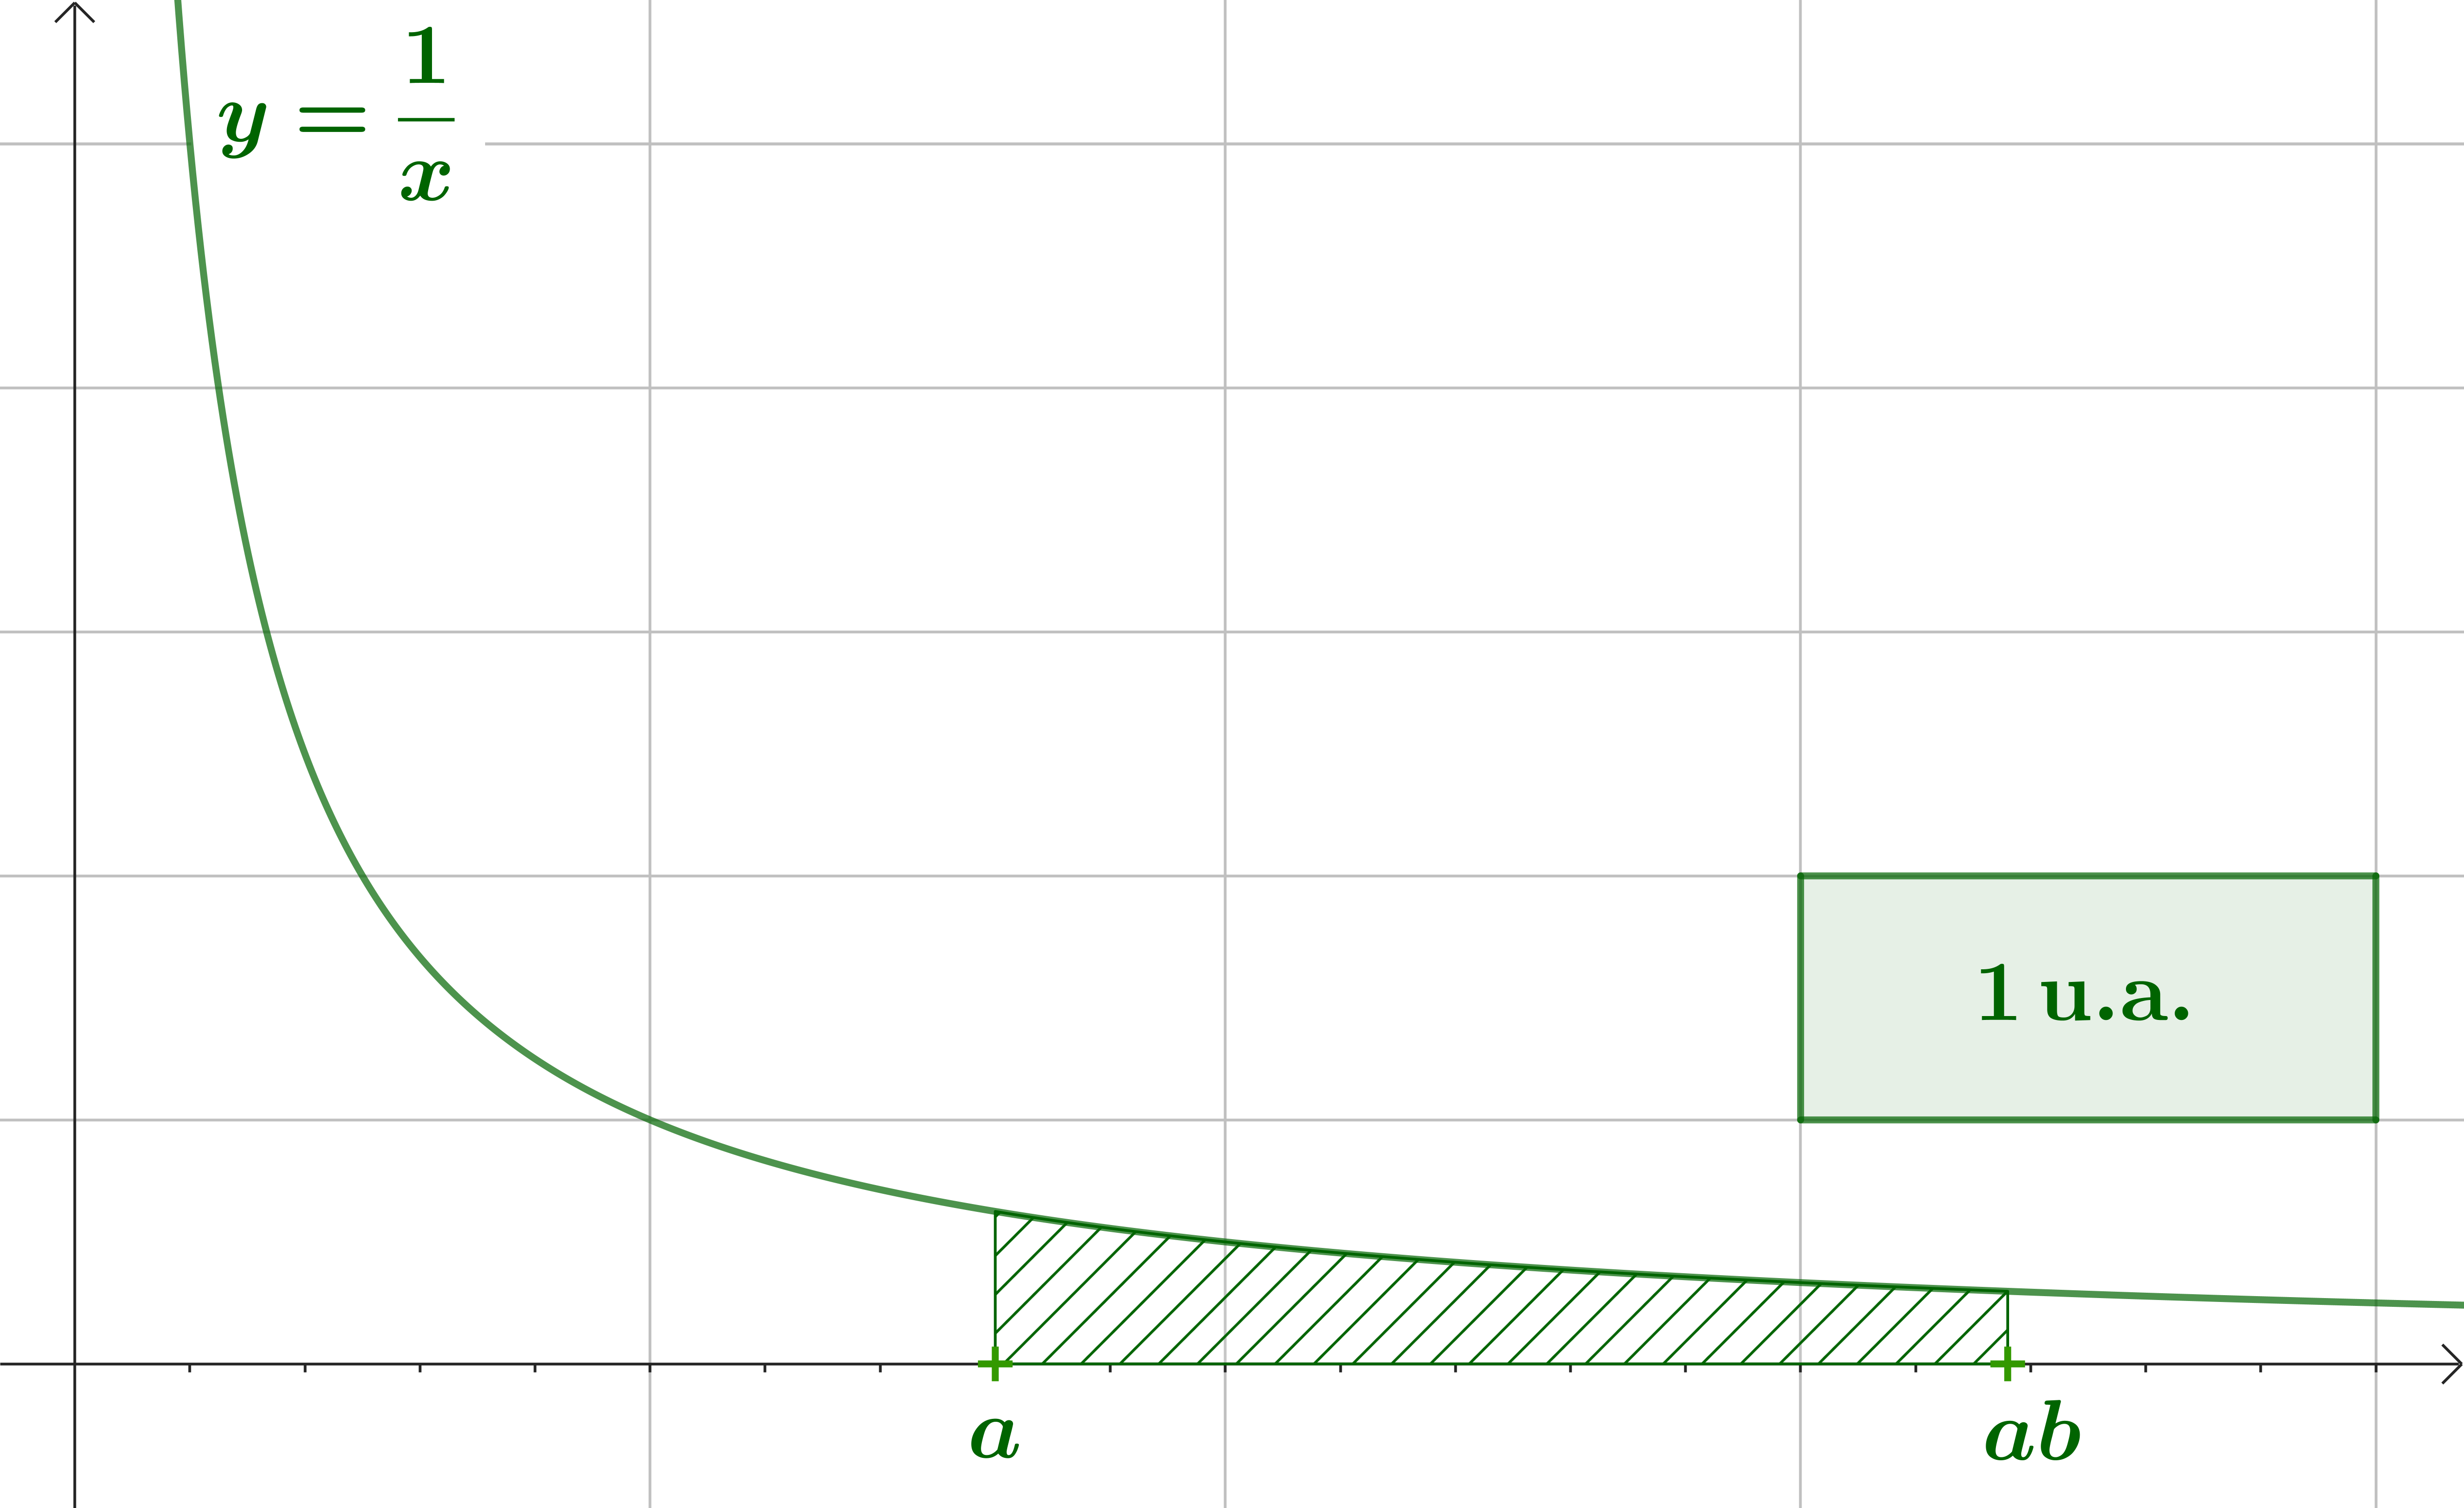
\includegraphics[scale=.5]{content/ln/func-eq-1.png}
    \end{center}

    Une dilatation horizontale $\phi$ de coefficient $\frac1a$ transforme $M(x_M ; y_M)$ en $M^{\,\prime}\big( \frac{x_M}{a} ; y_M)$.
    Appliquons $\phi$ à la surface associée à l'intégrale $\setproba{I}_{\,a}^{\,ab}$, ainsi qu'à la fonction inverse%
    \footnote{
        Noter l'abus de langage consistant à ne pas rappeler que nous travaillons juste sur $\RRsp$.
    }
    qui devient $f: x \mapsto \frac{1}{a x}$, puisque nous devons avoir $f(\frac{x}{a}) = \frac{1}{x}$.
    Il est important de noter qu'un rectangle d'une unité d'aire est transformé par $\phi$ en un rectangle de $\frac1a$ unité d'aire.

    \begin{center}
        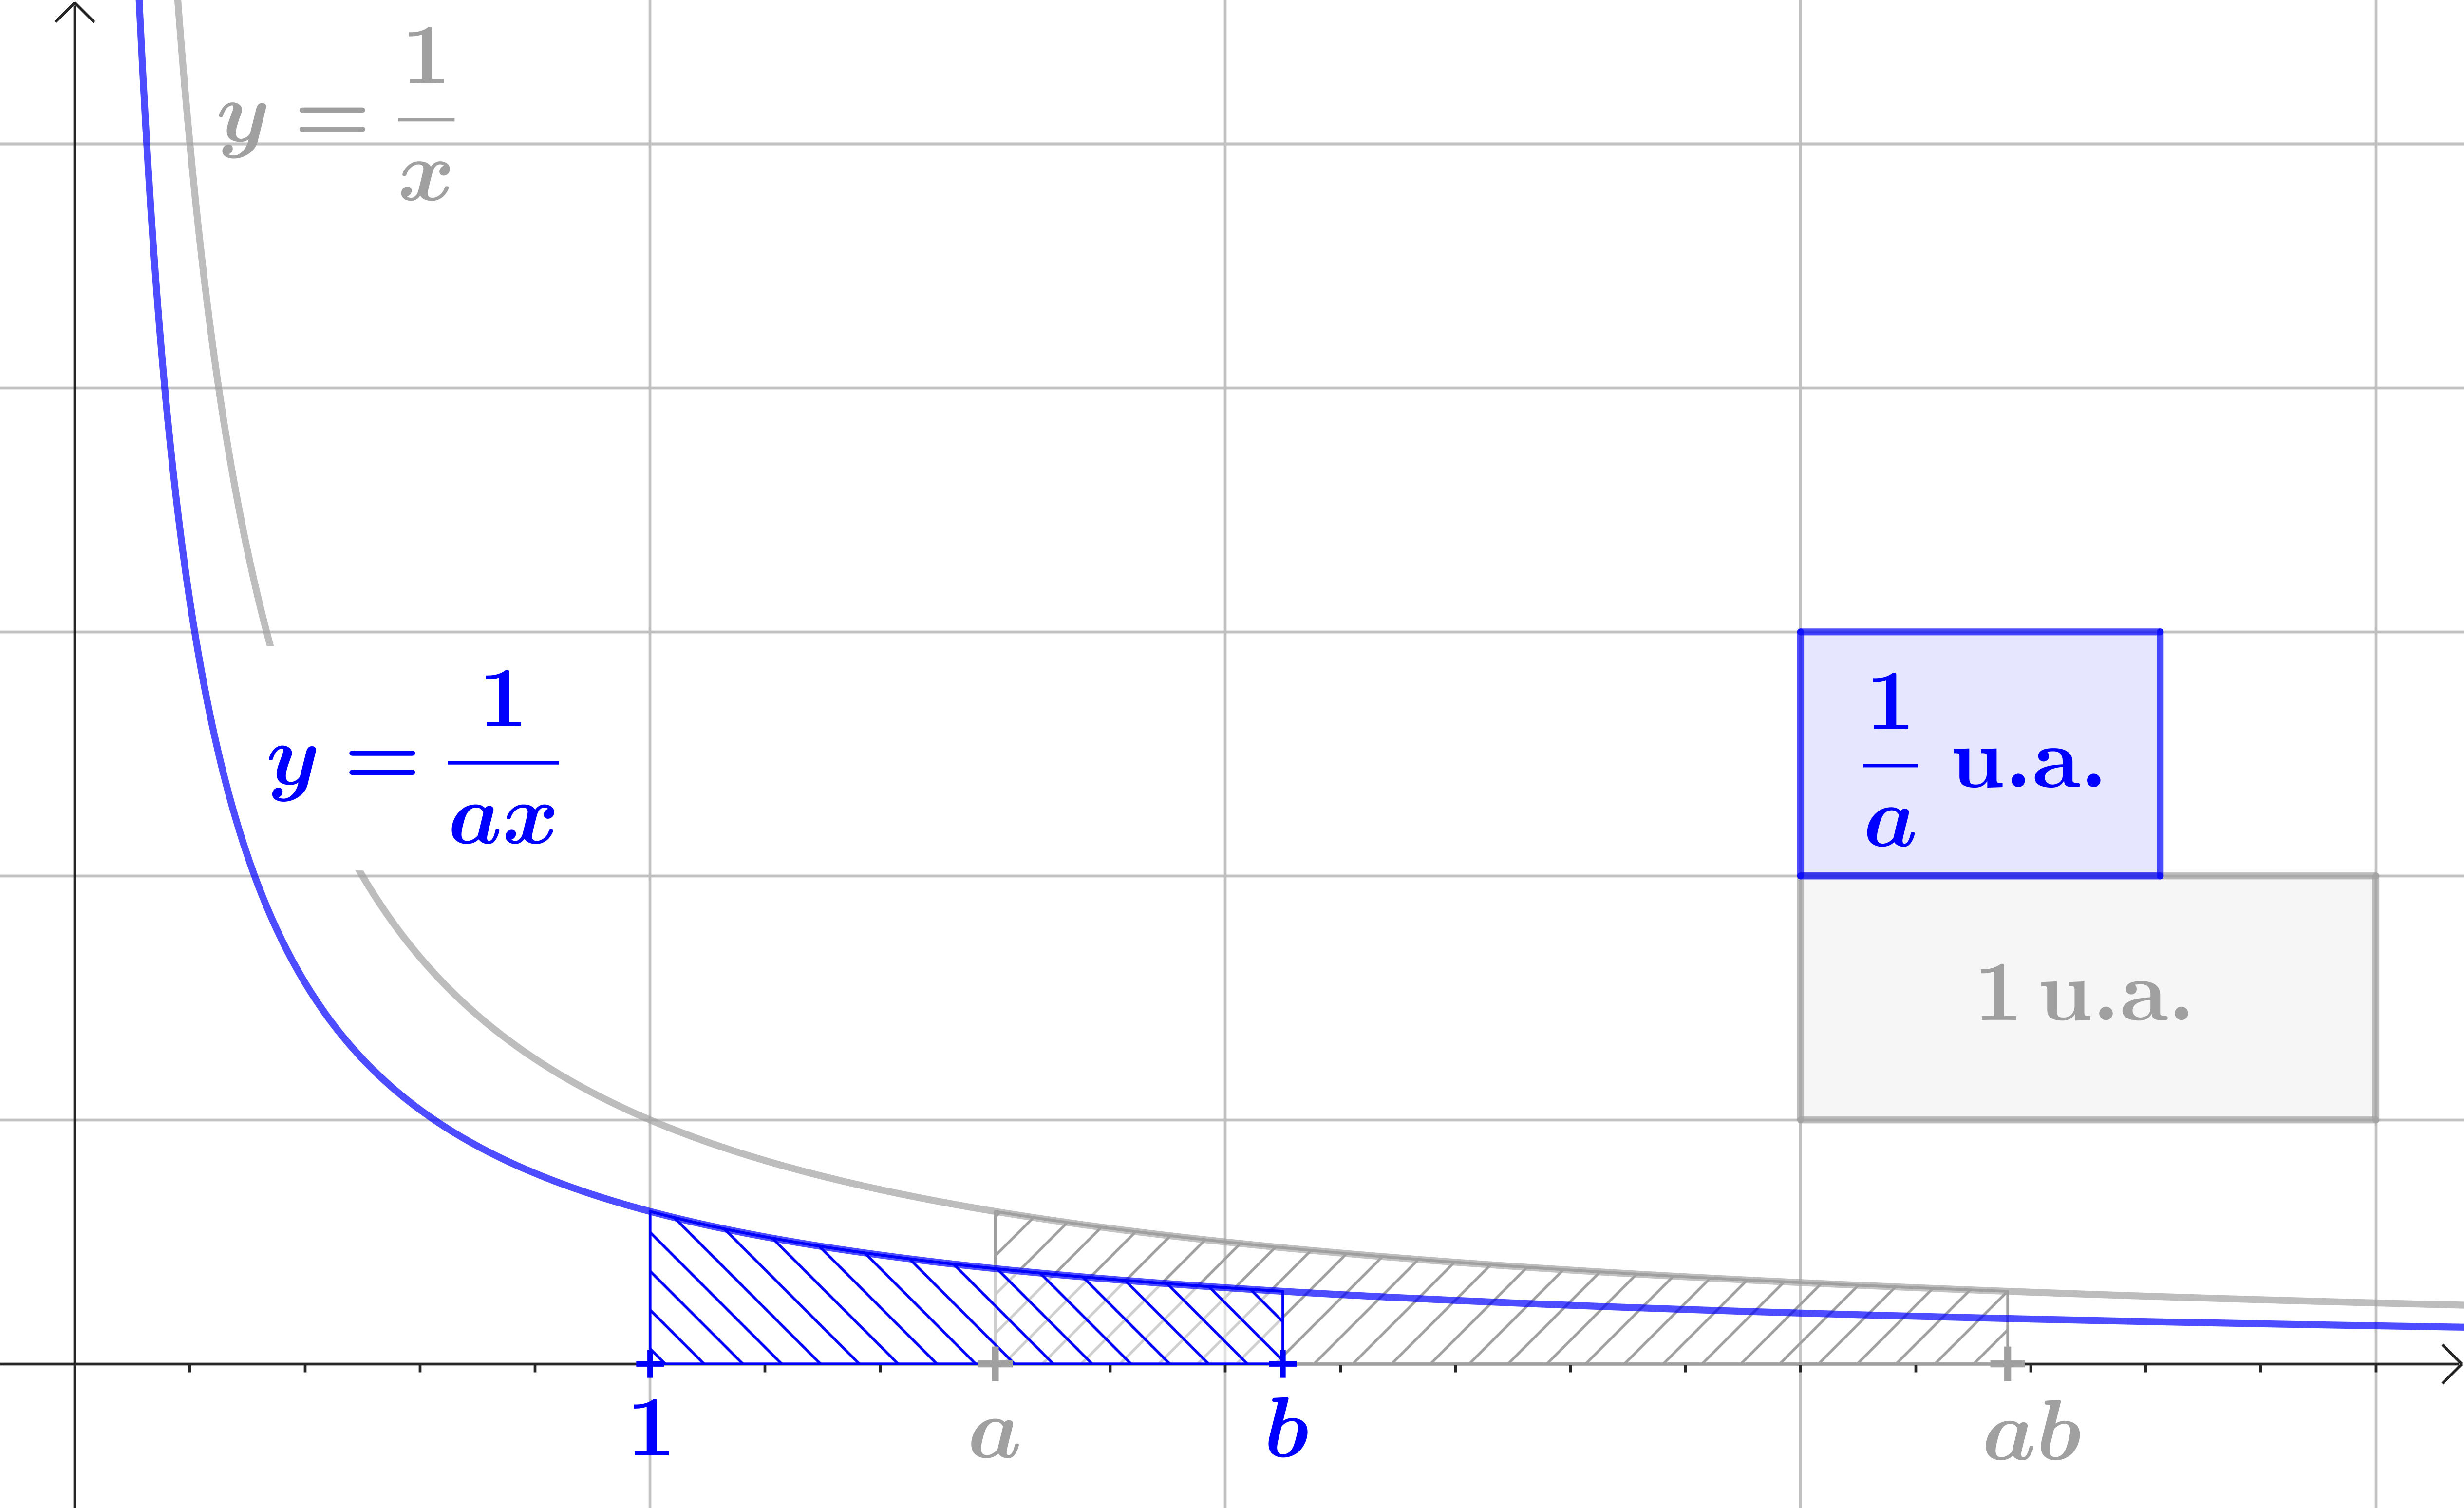
\includegraphics[scale=.5]{content/ln/func-eq-2.png}
    \end{center}

    Une dilatation verticale $\psi$ de coefficient $a$ transforme $M(x_M ; y_M)$ en $M^{\,\prime}\big( x_M ; a y_M)$.
    Appliquons $\psi$ à la surface associée à l'intégrale $\integrate*{\frac{1}{at}}{t}{1}{b}$, ainsi qu'à la fonction $f$ qui devient la fonction inverse. Notons qu'un rectangle de $\frac1a$ unité d'aire est transformé par $\psi$ en un rectangle d'une unité d'aire.

    \begin{center}
        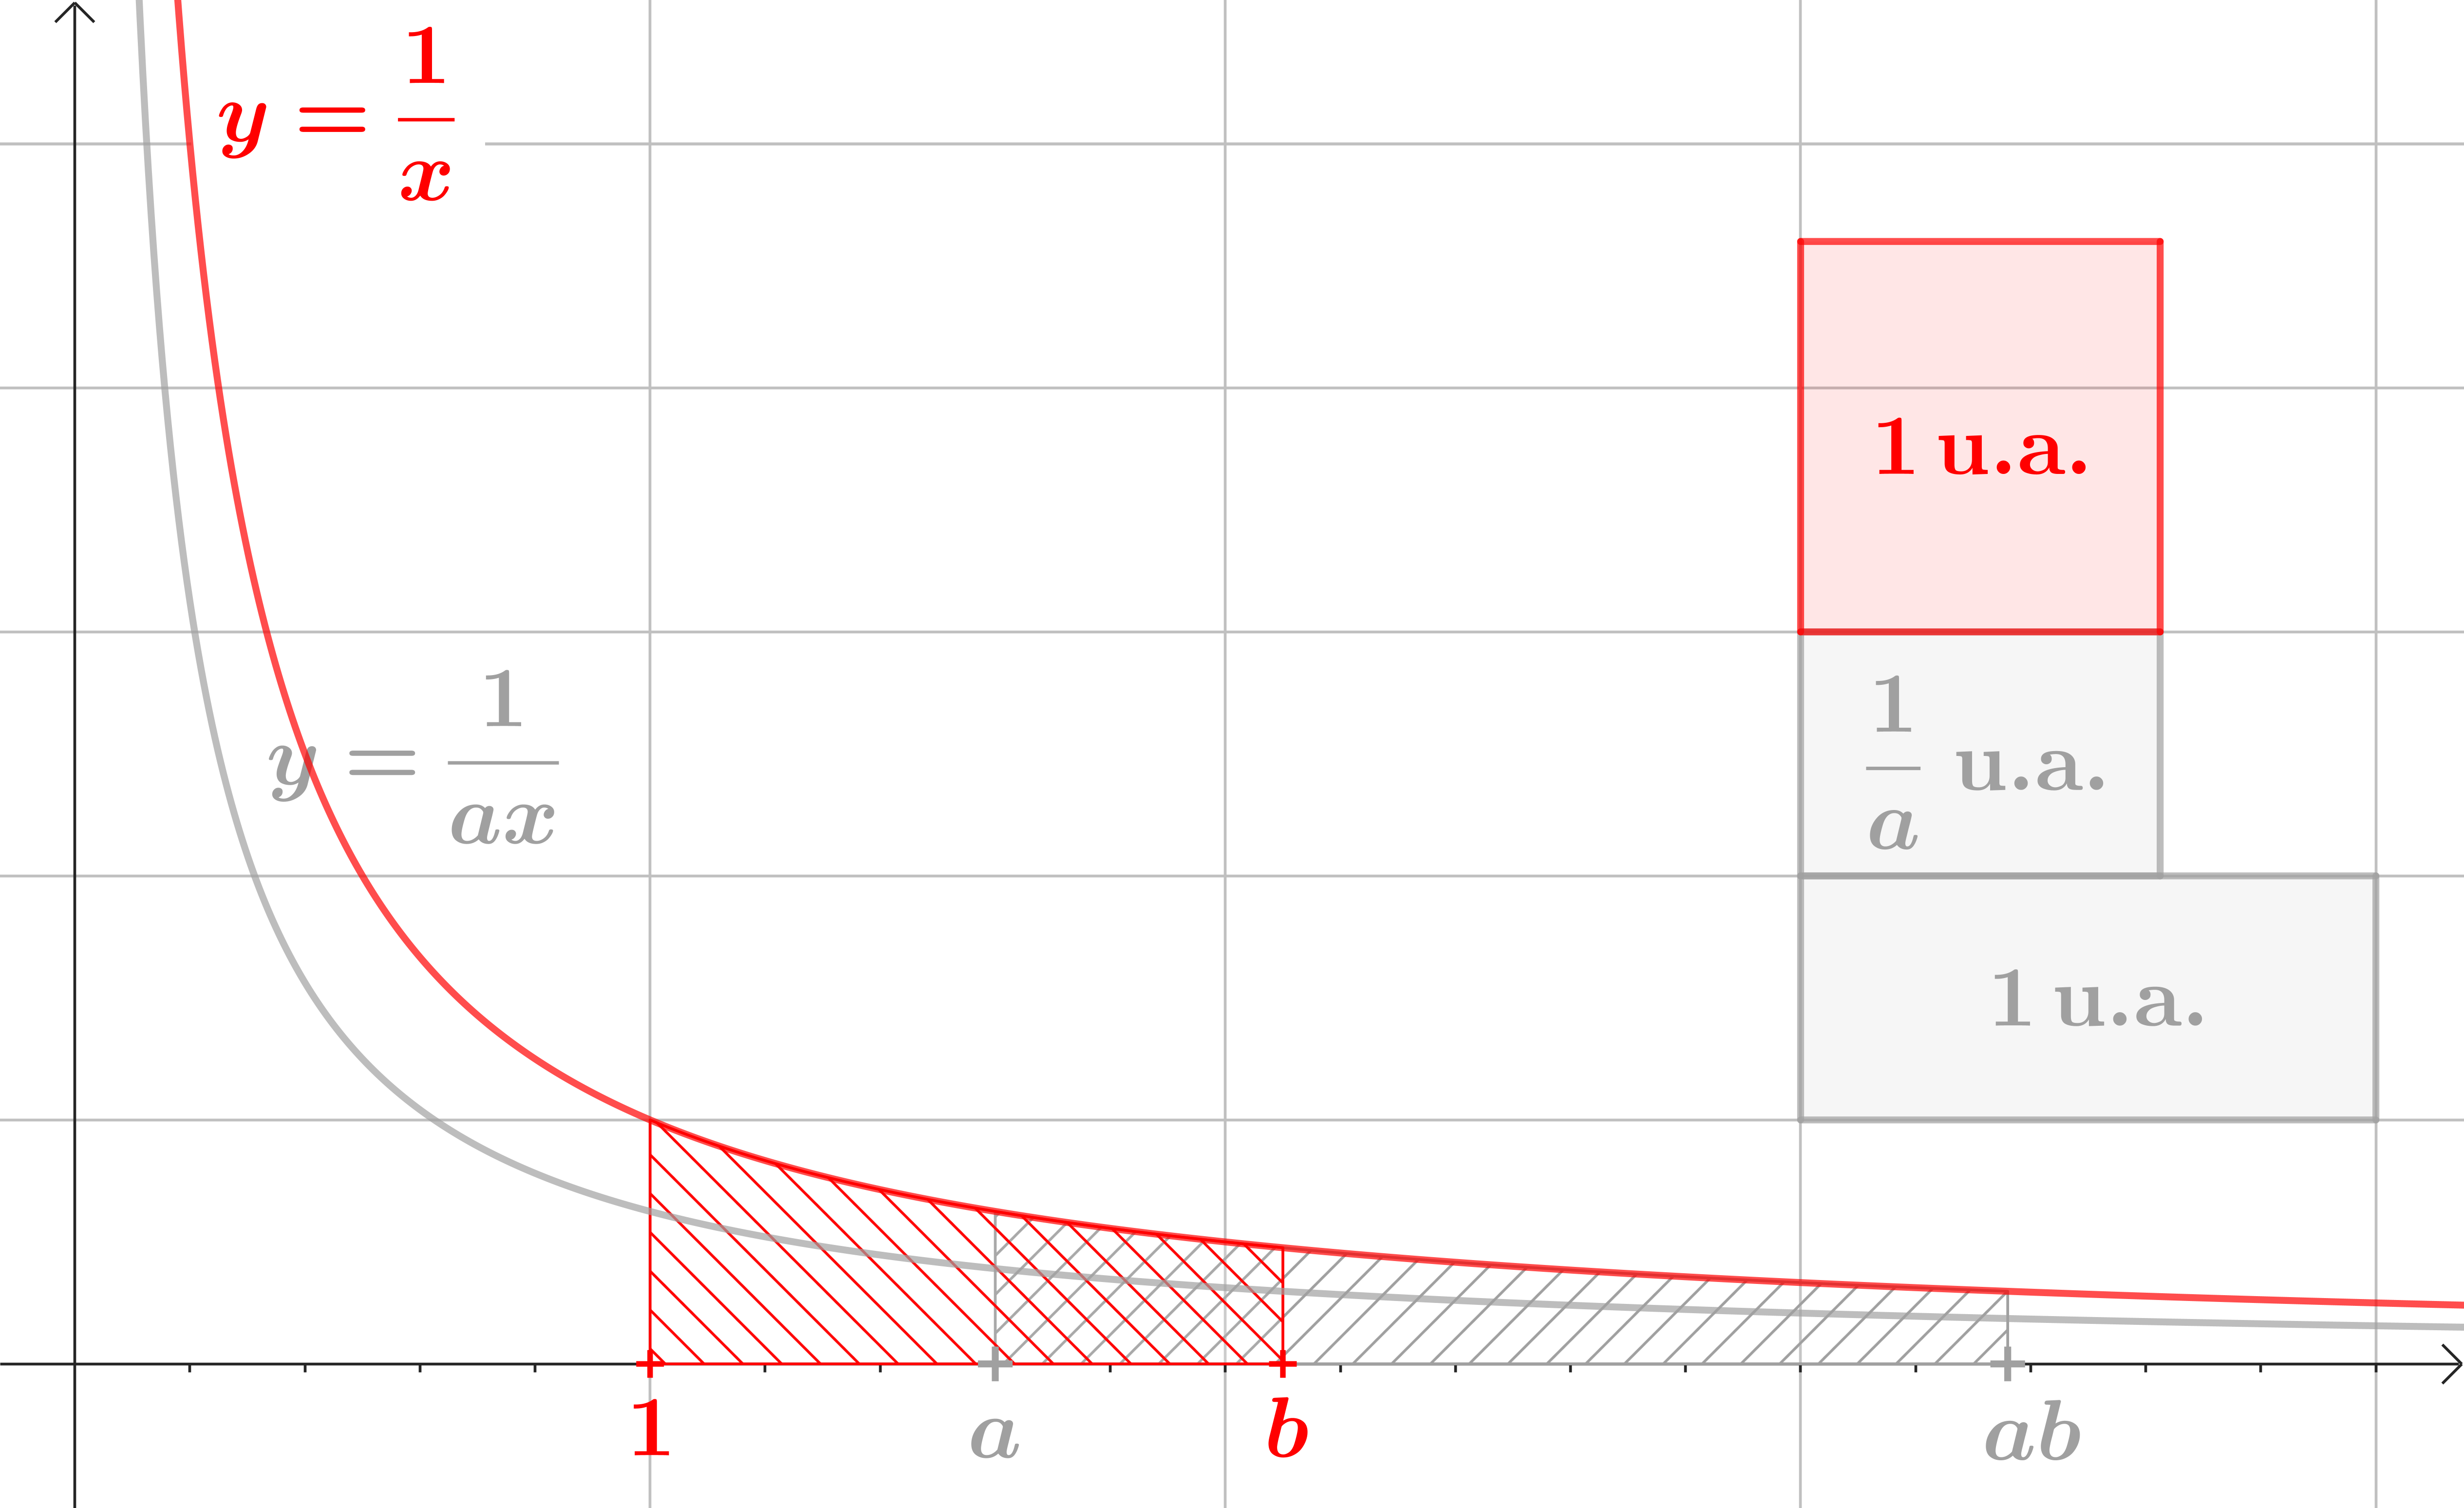
\includegraphics[scale=.5]{content/ln/func-eq-3.png}
    \end{center}

    Nous venons de justifier que
    $\setproba{I}_{\,a}^{\,ab} = \integrate*{\frac{1}{t}}{t}{1}{b}$,
    soit
    $\ln(a b) = \ln a + \ln b$,
    lorsque $1 < a < b$.
    La généralisation à $0 < a \leq b$ ne pose aucune difficulté.
\end{proof}


\begin{remark}[Aux bourbakistes]
    Ce qui a été dit ci-dessus se rédige rigoureusement, sans aucun souci, via des sommes de Riemann, par exemple.%
    \footnote{
        N'oublions pas que nous disposons d'au moins trois jolies théories de l'intégration:
        celle de Riemann,
        celle de Lebesgues,
        et
        la merveilleuse théorie de Kurzweil et Henstock.
    }
    La démonstration suivante ne souffre d'aucun doute, mais la donner sans plus d'explication serait bien dommage (la première approche évite toute interprétation mystique de l'équation fonctionnelle $\ln(a b) = \ln a + \ln b$).
\end{remark}


{
\emph{\altproof{}}
    Nous allons justifier que
    $\forall (a;b) \in ( \RRsp )^2$,
    $\ln(a b) = \ln a + \ln b$
    uniquement via l'analyse réelle.
    Comme les propriétés de la fonction $\ln$ nécessitent d'avoir une seule variable,
    il devient naturel de fixer $a \in \RRsp$, puis de considérer la fonction
    $f: \RRsp \to \RR$
    définie par
    $f(x) = \ln(a x) - \ln a - \ln x$.
    %
    La seule possibilité qui s'offre à nous est de dériver:
    $\der{f}{x}{1}(x) = a \cdot \frac{1}{a x} - \frac1x = 0$.
    %
    Or,
    une fonction de dérivée nulle sur un intervalle $I$ est forcément constante sur $I$,
    donc
    $\forall x \in \RRsp$,
    $f(x) = f(1)$,
    soit
    $f(x) = 0$.
    %
    Mission accomplie!
\qed
}


% ----------------------- %


\begin{fact} \label{ln-id}
    $\forall (a;n) \in \RRsp \times \ZZ$,
    nous avons
    $\ln(a^n) = n \ln a$,
    et
    $\ln(\frac1a) = - \ln a$.
\end{fact}


\begin{proof}
    De $\ln(a \cdot \frac1a) = \ln a + \ln(\frac1a)$, nous déduisons $\ln(\frac1a) = - \ln a$.
    %
    Quant à l'identité $\ln(a^n) = n \ln a$, une récurrence donne le résultat sur $\NN$, puis $\ln(a^{-n}) = -\ln(a^n)$ permet d'élargir à $\ZZsn$.
\end{proof}
